\section{Wi-Fi Monitoring}\label{Wireless Monitoring Metrics}

 Active and passive techniques have their advantages and disadvantages. In the following, we outline the main characteristics of each one of them. Each of the techniques will be best-suited depending on the  goal and context of the experiment.

\subsection{Active}

Active measurement is a technique in which traffic is injected in the network to get a sense of the network status. The injected packets are called probes. For our work we use active measurements to obtain metrics on bandwidth, Round-Trip Time (RTT) and packet loss. In the Wi-Fi context, bandwidth active measurements can help to identify where the bottleneck is happening. We have also used active bandwidth measurement tools to generate traffic in our experimental setup to resemble real-case scenarios. High RTT can help to identify if congestion is happening in the home Wi-Fi. In a similar way, packet loss can denote interference as frames are destroyed in the Wi-Fi link. While working with active measurements it is  important to pay attention to the probes size and probing rate. Large probe sizes and aggressive probing rate can cause overhead. Overhead does not only disrupts user traffic but can also lead to biased measurements. In the following bullet points we outline the strengths and weaknesses of active measurements that we consider relevant for our work. We also include the ones we work with for this paper.


\textbf{Strengths}
\begin{itemize}
	\item Full ownership of the network is not required.
	\item They do not require large space to store data collected as generally, probe packets are small.
	\item Privacy concerns are minimal as probe packets used to measure are made of random data which has no sensitive information.
	\item Useful to get the state of the network on-demand.
\end{itemize}
	

\textbf{Weaknesses}
\begin{itemize}
	\item Overhead might occur if probe size and probing rate are chosen without due diligence of network conditions.
	\item Biased results can be obtained if probes, either size or rate, cause overhead in the network.
\end{itemize}


Under the scope of active measurement techniques, the following are the metrics to be actively collected for our work.

\begin{itemize}
	%\item One-Way Delay
	\item \textbf{Round Trip Time}
	\begin{itemize}
		\item For our goal, RTT can helps us identify if we are experiencing attenuation and interference in the home Wi-Fi. High RTT values can give a sense of latency in the home Wi-Fi which is potentially correlated to attenuation. Packet loss in the other hand, will point to interference related impairments as frames are being destroyed, causing the loss of these frames.
	\end{itemize}
	
	\item \textbf{Throughput}
	\begin{itemize}
		\item In Wi-Fi, throughput active measurement can assist to identify if congestion is happening in the Wi-Fi link. For example, if the AP reports a strong signal to the wireless client and minimal losses but the throughput is low, it is likely that the AP is experiencing congestion.
	\end{itemize}
	%\item \textbf{Losses}
	%\begin{itemize}
	%	\item ICMP reply packets not coming back to the source.
	%\end{itemize}
\end{itemize}

\subsection{Passive}

Passive measurement techniques rely on a ``sit and listen" approach. The instrument conducting passive measurements in the network sits in a specific location along the path and records the metrics of interest. The monitor can be a component of the network itself, for example a router. It can also be device devoted to measure, such as a wireless sniffer. An important difference between active and passive techniques is that the latter do not trigger probes. Overhead due to probe packets is not present in passive measurements. However, computational and storage resources in the passive measuring device can be important factors to consider. The device might require to have enough space to store the data being collected. In a similar way, the computational power of the device can be required to be high depending on the speed of the link being measured. A Gigabit link in a core router will handle significantly more data than an 100Mbps Ethernet link in an access switch. 
Outlined in the following list a high level summary of the key strength and weaknesses of passive measurement techniques for our work purposes. We also outline the ones we use for our work.

\textbf{Strength}
\begin{itemize}
	\item No extra traffic is generated to collect metrics, risk of causing overhead is minimized.
\end{itemize}


\textbf{Weaknesses}
\begin{itemize}
	\item Large storage capacity can be required to store collected data. Not all measuring devices have large storage capacity, i.e. Access Points.
	\item Access to equipment working as passive measurement device is required. This is not possible for most users at multiple devices along an Internet path.
	\item High computational power on the measuring device can be required depending on the link being monitored and data granularity pursued. Not all devices can provide high computational power, i.e. Access Points.
\end{itemize}

\begin{itemize}
	%\item \textbf{PHY Tx Rate}
	%\begin{itemize}
	%	\item The speed at which the device is connected to. Bitrate adaptation techniques are triggered based on channel conditions. Therefore this metric can assist to estimate the channel conditions.
	%\end{itemize}
	\item \textbf{RSSI - Received Signal Strength Indicator}
	\begin{itemize}
		\item In our experiments we collect the RSSI from the AP and the wireless client. The RSSI help us to identify if there is attenuation happening in the link. A low RSSI denotes attenuation in the wireless link.
		\item Low RSSI can be caused by poor AP placement due to large distance between wireless client and AP or, obstacles between both.
	\end{itemize}
	%\hfill \break
	%\item \textbf{Busy Time}
	%\begin{itemize}
		%\item This metric is associated to the time the channel was busy, in other words the time channel was being used and therefore not eligible for data exchange. Reasons for channel busy time to be close to 100\% can be contention by other Wi-Fi devices or interference from non-Wi-Fi sources.
	%\end{itemize}
	
	\item \textbf{PHY Tx Rate}
	\begin{itemize}
		\item The PHY Tx Rate at the wireless nodes can be an indicator of poor Wi-Fi link quality. A low PHY Tx Rate can help to diagnose a congestion, attenuation or interference Wi-Fi impairment. In collaboration with other metrics the scope of the impairment can be narrowed down.
		\item For example, if the RSSI is strong, meaning there is no attenuation; loss rate is minimal, meaning interference is not present, but Tx PHY Rate is low; the impairment scope can be narrowed down to congestion.
	\end{itemize}
	
	\item \textbf{Noise}
	\begin{itemize}
		\item  Noise measurements assist know if environment where the wireless client or the AP is placed is suitable for Wi-Fi. For example, if the noise level at a particular wireless client is high, we expect that node to be the only one with Wi-Fi degraded quality. In the other hand, if the AP is the one sensing high noise levels, we can expect all the clients connected to that AP to experience degraded Wi-Fi.
		\item Noise can be caused by devices which ``do not speak Wi-Fi language" such as microwave ovens, cordless phones and similar. Noise can help to distinguish between congestion and interference. Unlike congestion, interference is driven by non-WiFi sources.
	\end{itemize}
	
	\item \textbf{Throughput - Driver Logs}
	\begin{itemize}
		\item The throughput from the driver logs assist us to sense a Wi-Fi impairment. Low throughput can be an indicator of congestion, attenuation or interference.
		\item In a similar way as for actively measuring throughput,  collaborating with other metrics can narrow down the potential Wi-Fi impairment.
		\item Additionally, passively measuring bandwidth helps to validate we obtain similar values obtained from active measurement techniques.
	\end{itemize}
	\newpage
	\item \textbf{Frame Delivery Ratio}
	\begin{itemize}
		\item Frame Delivery Ratio depicts the ratio between packets successfully received and total packets sent. The FDR metric can assist to get a sense of link quality. Low FDR indicates poor link quality. 
		\item Poor link quality can be caused due to congestion, attenuation or interference. In a similar way as with other metrics in our work, we collaborate with other metrics to narrow down the potential Wi-Fi impairment being experienced.
	\end{itemize}

\end{itemize}

The metrics described before have been collected from different devices in our setup. Previous works have identified that even with similar wireless conditions devices can experience different throughput and bitrates \cite{measuring_user_traffic}, therefore we use different vantage points. Passive metrics have mostly been collected at the wireless client and AP. We extract these metrics from driver logs and derived statistic from them. Additionally we setup a wireless sniffer to get wireless captures. We use the wireless captures to validate the values we get from the logs at wireless client and AP. In the case of active metrics, we collect them from a wired client. The wired client works as the device in which we target to deploy our tool. From the wired client we trigger the active probing tool to collect RTT and throughput. The RTT measurements are collected using a custom ping-like tool. The active throughput is collected with \emph{iPerf}. In section \ref{Wireless Bottleneck Detector} we share instrumentation details on the tools we use to obtain the metrics we work with.

\subsection{Finding the probing rate}\label{probing_rate}

Finding the probing rate is important when working with active measurements. A high rate can cause overhead, whereas a low rate can fail to capture the status of the network. To approach this challenge we conducted experiments in our office lab. Our experiments consisted in sending a series of ping trains which included multiple pings inside each train. We ran the tests with different train inter-spacing values and with different amount of pings inside the trains. The first finding from our experiments was a delay in RTT due to power save mode in devices. The power save mode sends the NIC to sleep. We refer to this delay as the ``sleeping NIC". We found that when the inter-train spacing is smaller or equal to 100 msec the power save mode delay is not present. Based on this finding we set our lower bound for inter-train spacing to 100 msec. We set our upper bound to 1000 msec as the RTT within a single-hop home Wi-Fi  network without significant cross-traffic is expected to be only a few milliseconds. This observation is remarked in the work of Sundaresan et al. \cite{homeoraccesslink}.

The second relevant finding is associated to the RTT value of each ping within a train. We found that even with inter-train spacing values above 100 msec it is possible to overcome sleeping NIC delay by considering the RTT value of the 3rd or greater ping within a train. We noticed that the RTT value for ping greater or equal to the 3rd ping in a train depicted similar RTT values as when the sleeping NIC delay is not present. After these observations we defined our baseline to be 100 msec inter-train spacing and 3 pings per train. Figure \ref{image:Avg_RTT_Three_Pings} illustrates the values for the average round trip time of three pings in a train. The inter-ping spacing is equally distributed among the number of pings in a train and depends on the inter-train spacing. For example, the inter-ping spacing value for 3 pings in a 100 msec inter-train series is 100 msec/3 or ~33.33 msec.

\begin{figure}[h]
	\centering
	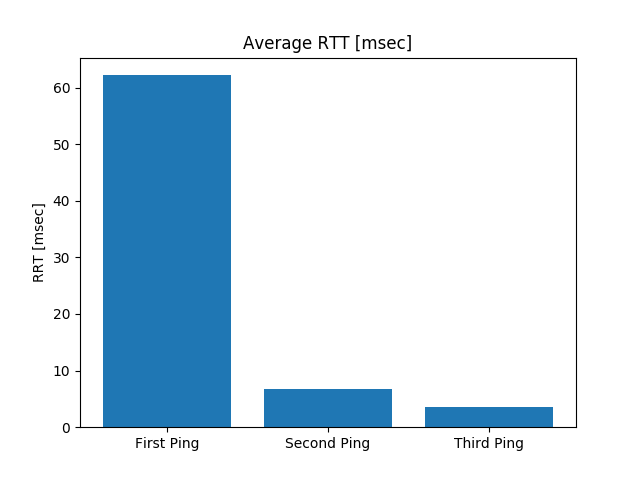
\includegraphics[width=8cm]{Three_Pings/Three_Pings_Avgs}
	\caption{Average RTT for Three Ping Series}
	\label{image:Avg_RTT_Three_Pings}
\end{figure}

With this exercise we defined our baseline, we implemented similarity tests between our baseline results and samples derived from the baseline. We refer to our baseline as aggressive probing. To keep the samples to follow the same distribution as our baseline we implemented a Poisson process to generate the inter-train space intervals. In other words, randomly sampling from a Poisson process will result in another Poisson-distributed process \cite{raikov_decomposition}. This feature has been included in our GoPing tool. We sampled our baseline to obtain from 10\% to 90 \% of our original data points. We implemented Bernoulli random sampling to extract our samples. Finally, we ran Two-sample Kolmogorov-Smirnov tests between our baseline and samples. From the results we noticed that the sample which delivers a similar ECDF to our baseline is the one that keeps 50\% of the original baseline data points. Figure \ref{image:ECDF_aggressive_vs_sampling} illustrates both ECDFs.

\begin{figure}[h]
	\centering
	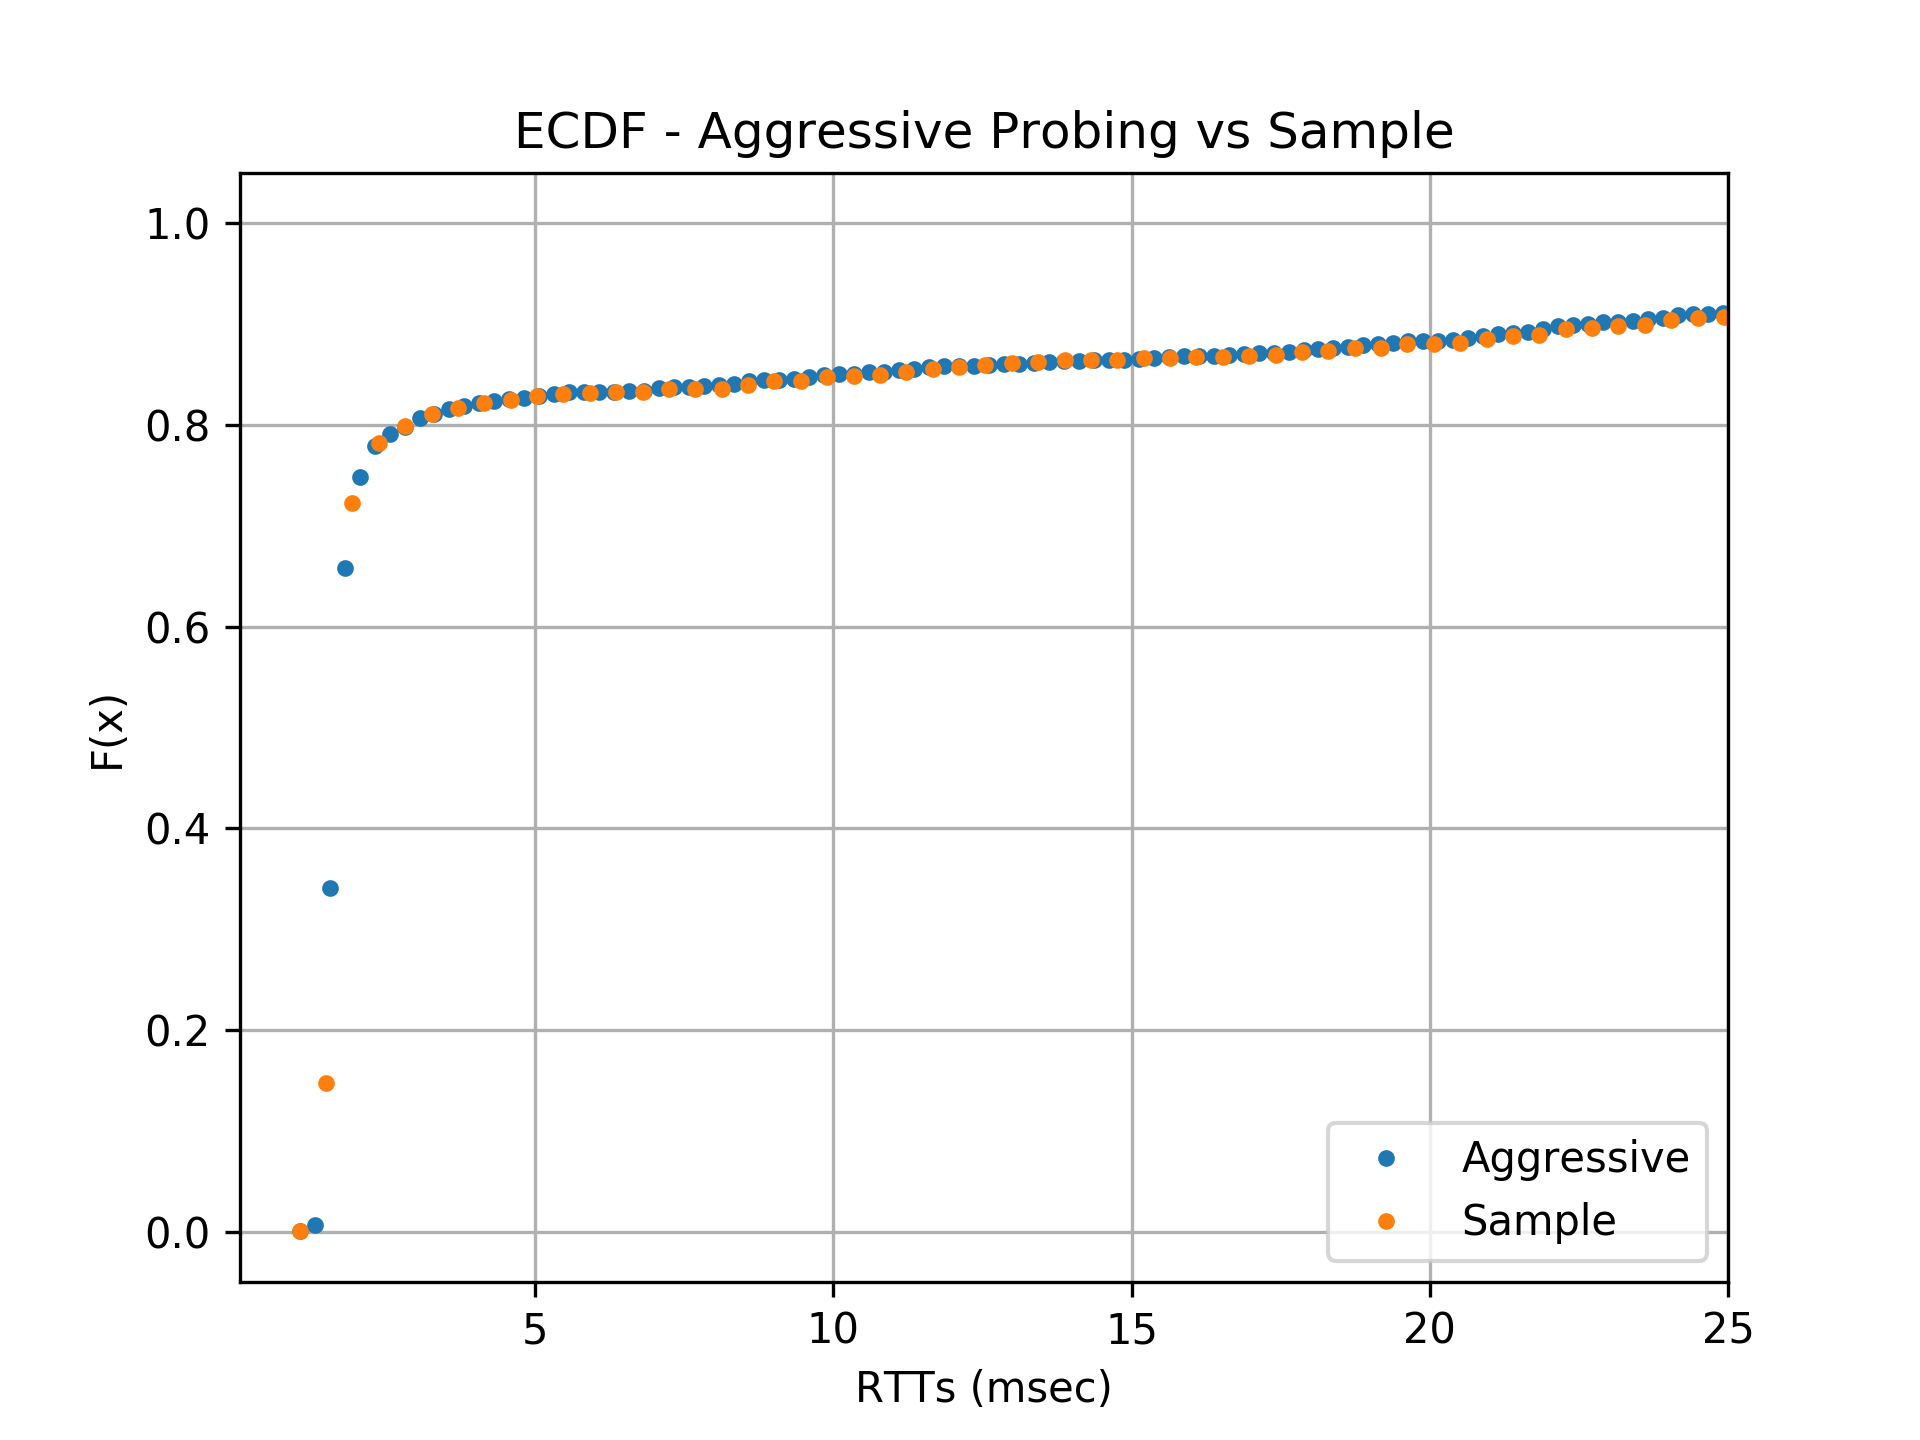
\includegraphics[width=8cm]{ECDF_Similarity/Aggressive_vs_Sample_Probing}
	\caption{ECDF - Aggressive Probing vs Sample}
	\label{image:ECDF_aggressive_vs_sampling}
\end{figure}

In figure \ref{image:ECDF_aggressive_vs_sampling} we can see the overlap between the sample keeping 50\% of original data points and the original baseline derived from aggressive probing. This was the sample in which the overlap occurred, based on this result we set our active probing rate. As the RTT ECDF of the sample with half of the original data is similar to the original baseline, we set our probing rate to be 200 msec.

After finding the active probing rate as described in Section \ref{probing_rate} we tested it in the testbed where we ran our experiments. Further description on our labs setup is covered in Section \ref{labs_setup}. The tests consisted in sending as many batches as possible for 10 min at 100 and 200 msec probing rates. Additionally we varied the attenuation with values of 0, 15 and 30 dBm. Table \ref{table:Att_Rate_Test_Values} summarizes the values used for the test. The test sessions took place in the 2.4 GHz band using 802.11n WLAN with no authentication. We ran each experiment session 5 times, in total we obtained 30 samples.

\begin{table}[h]
	\begin{center}
		\begin{tabular}{||c c||}
			\hline
			Attenuation & Probing Rate\\ [0.5ex] 
			\hline\hline
			0 dBm & 100msec\\ 
			\hline
			0 dBm & 200msec\\
			\hline
			15 dBm & 100msec\\
			\hline
			15 dBm & 200msec\\
			\hline
			30 dBm & 100msec\\
			\hline
			30 dBm & 200msec\\ [1ex] 
			\hline
		\end{tabular}
	\end{center}
	\caption{Attenuation and Probing Rate Validation Values}
	\label{table:Att_Rate_Test_Values}
\end{table}

We compared the RTT ECDF of both to check similarity between probing rates. The expectation was for curves to be similar to each other. As expected, figure \ref{fig:att_0_100and200msec} illustrates the similarity between both RTT ECDF probing rates. The next expected behavior was for RTT to increase as the attenuation values increases. Figure \ref{fig:rate_200msec_Att_0_15_30dBm} help us to validate the expected behavior. As we increase attenuation, RTT increases.

\begin{figure*}[t]
	\begin{subfigure}[t]{.53\textwidth}
		\centering
		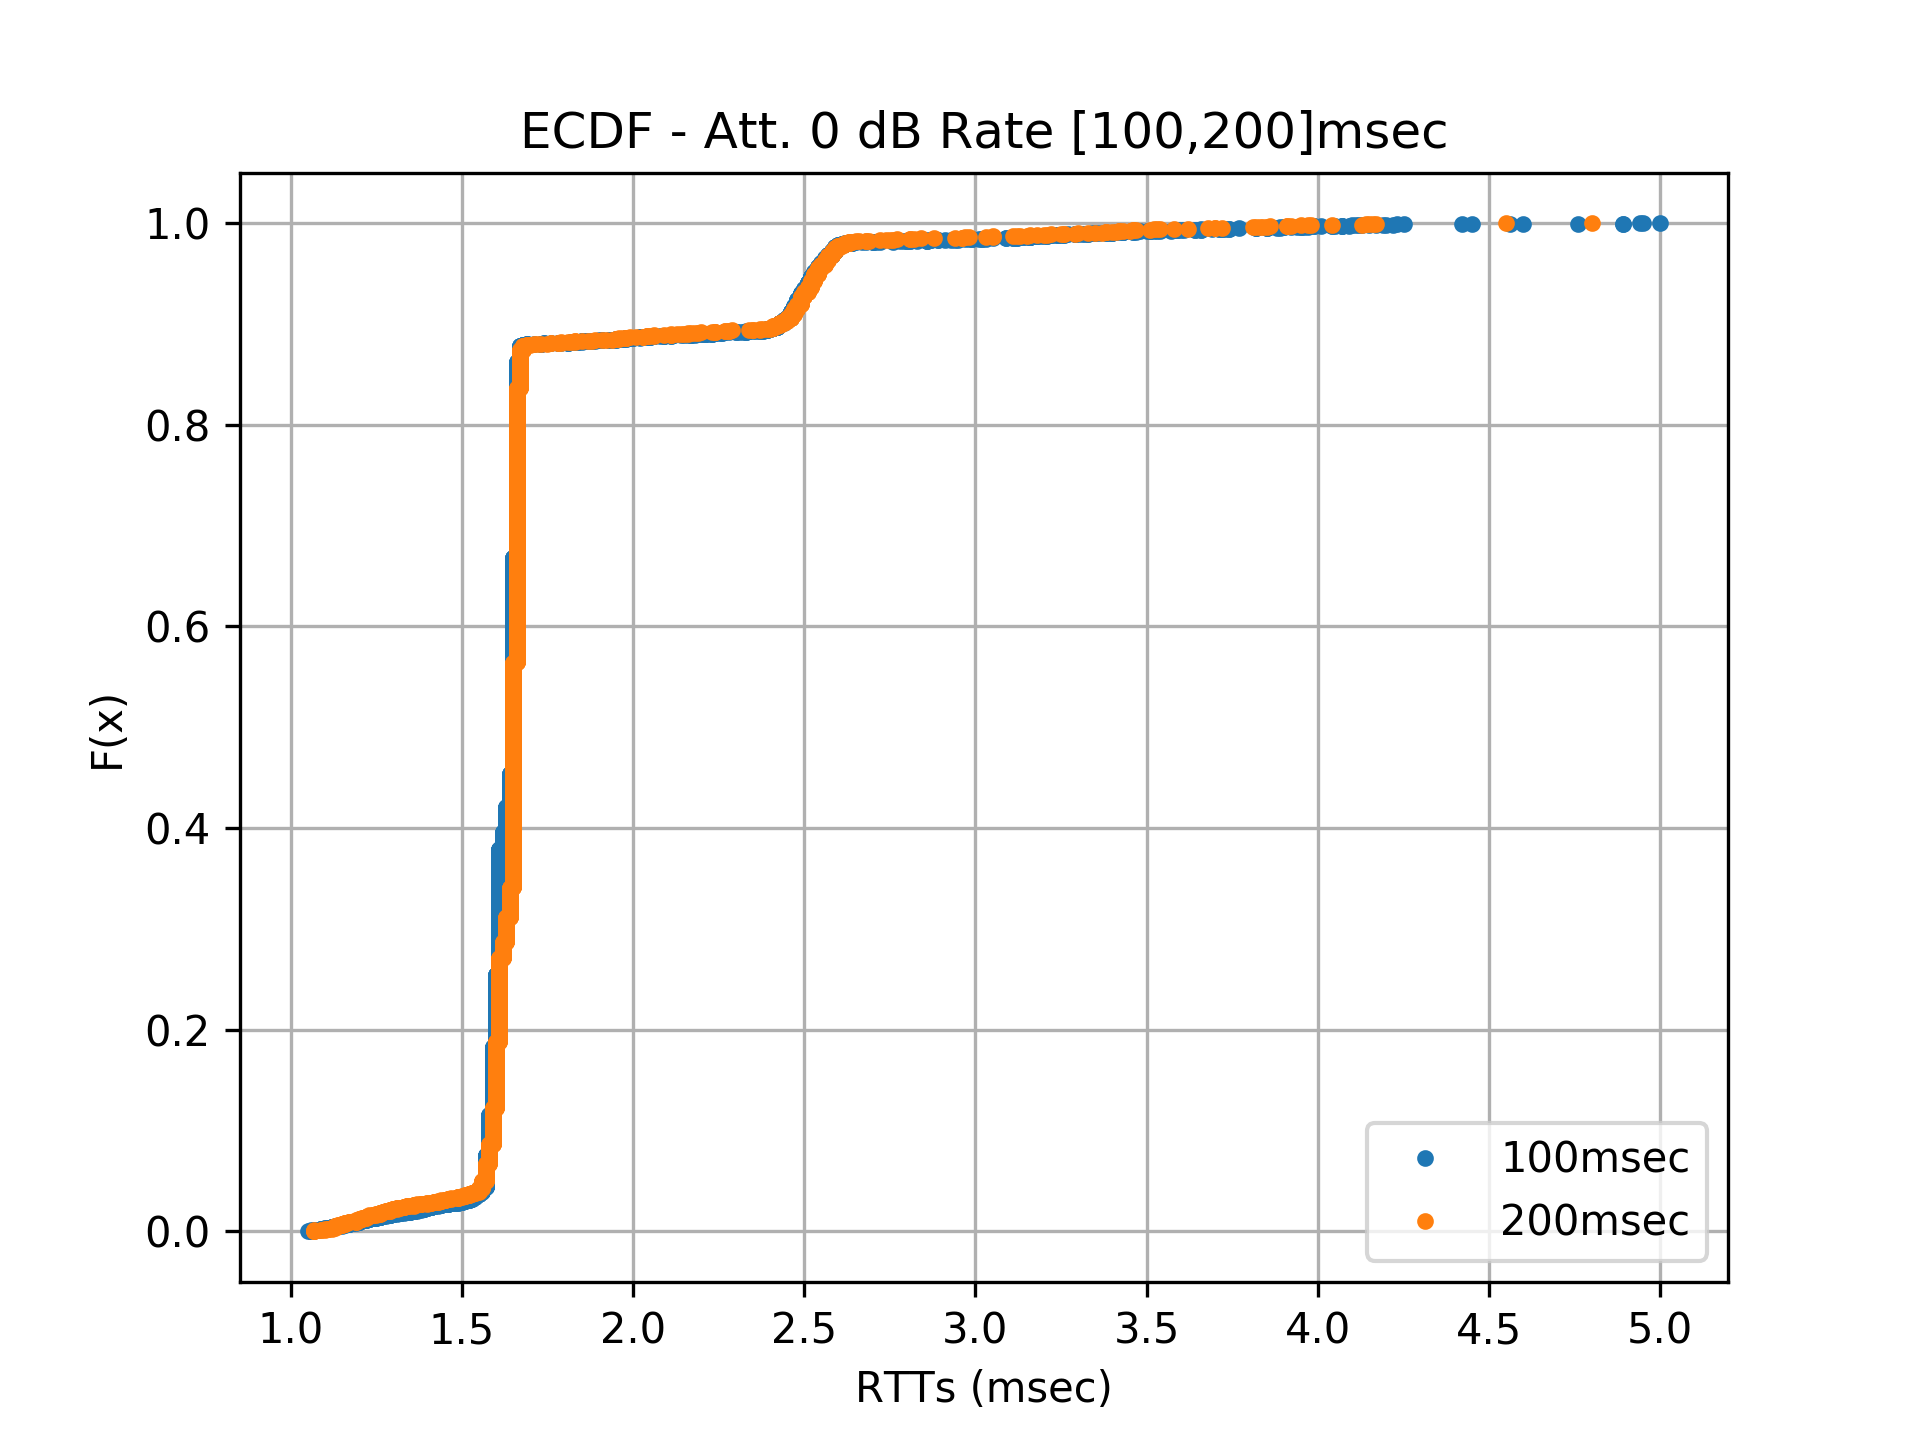
\includegraphics[width=.9\textwidth]{Rates_Atts/Att_0dBRate[100,200]msec}
		\caption{Att. 0 dBm - Rate 100,200 msec}
		\label{fig:att_0_100and200msec}
	\end{subfigure}\hfill
	\begin{subfigure}[t]{.53\textwidth}
		\centering
		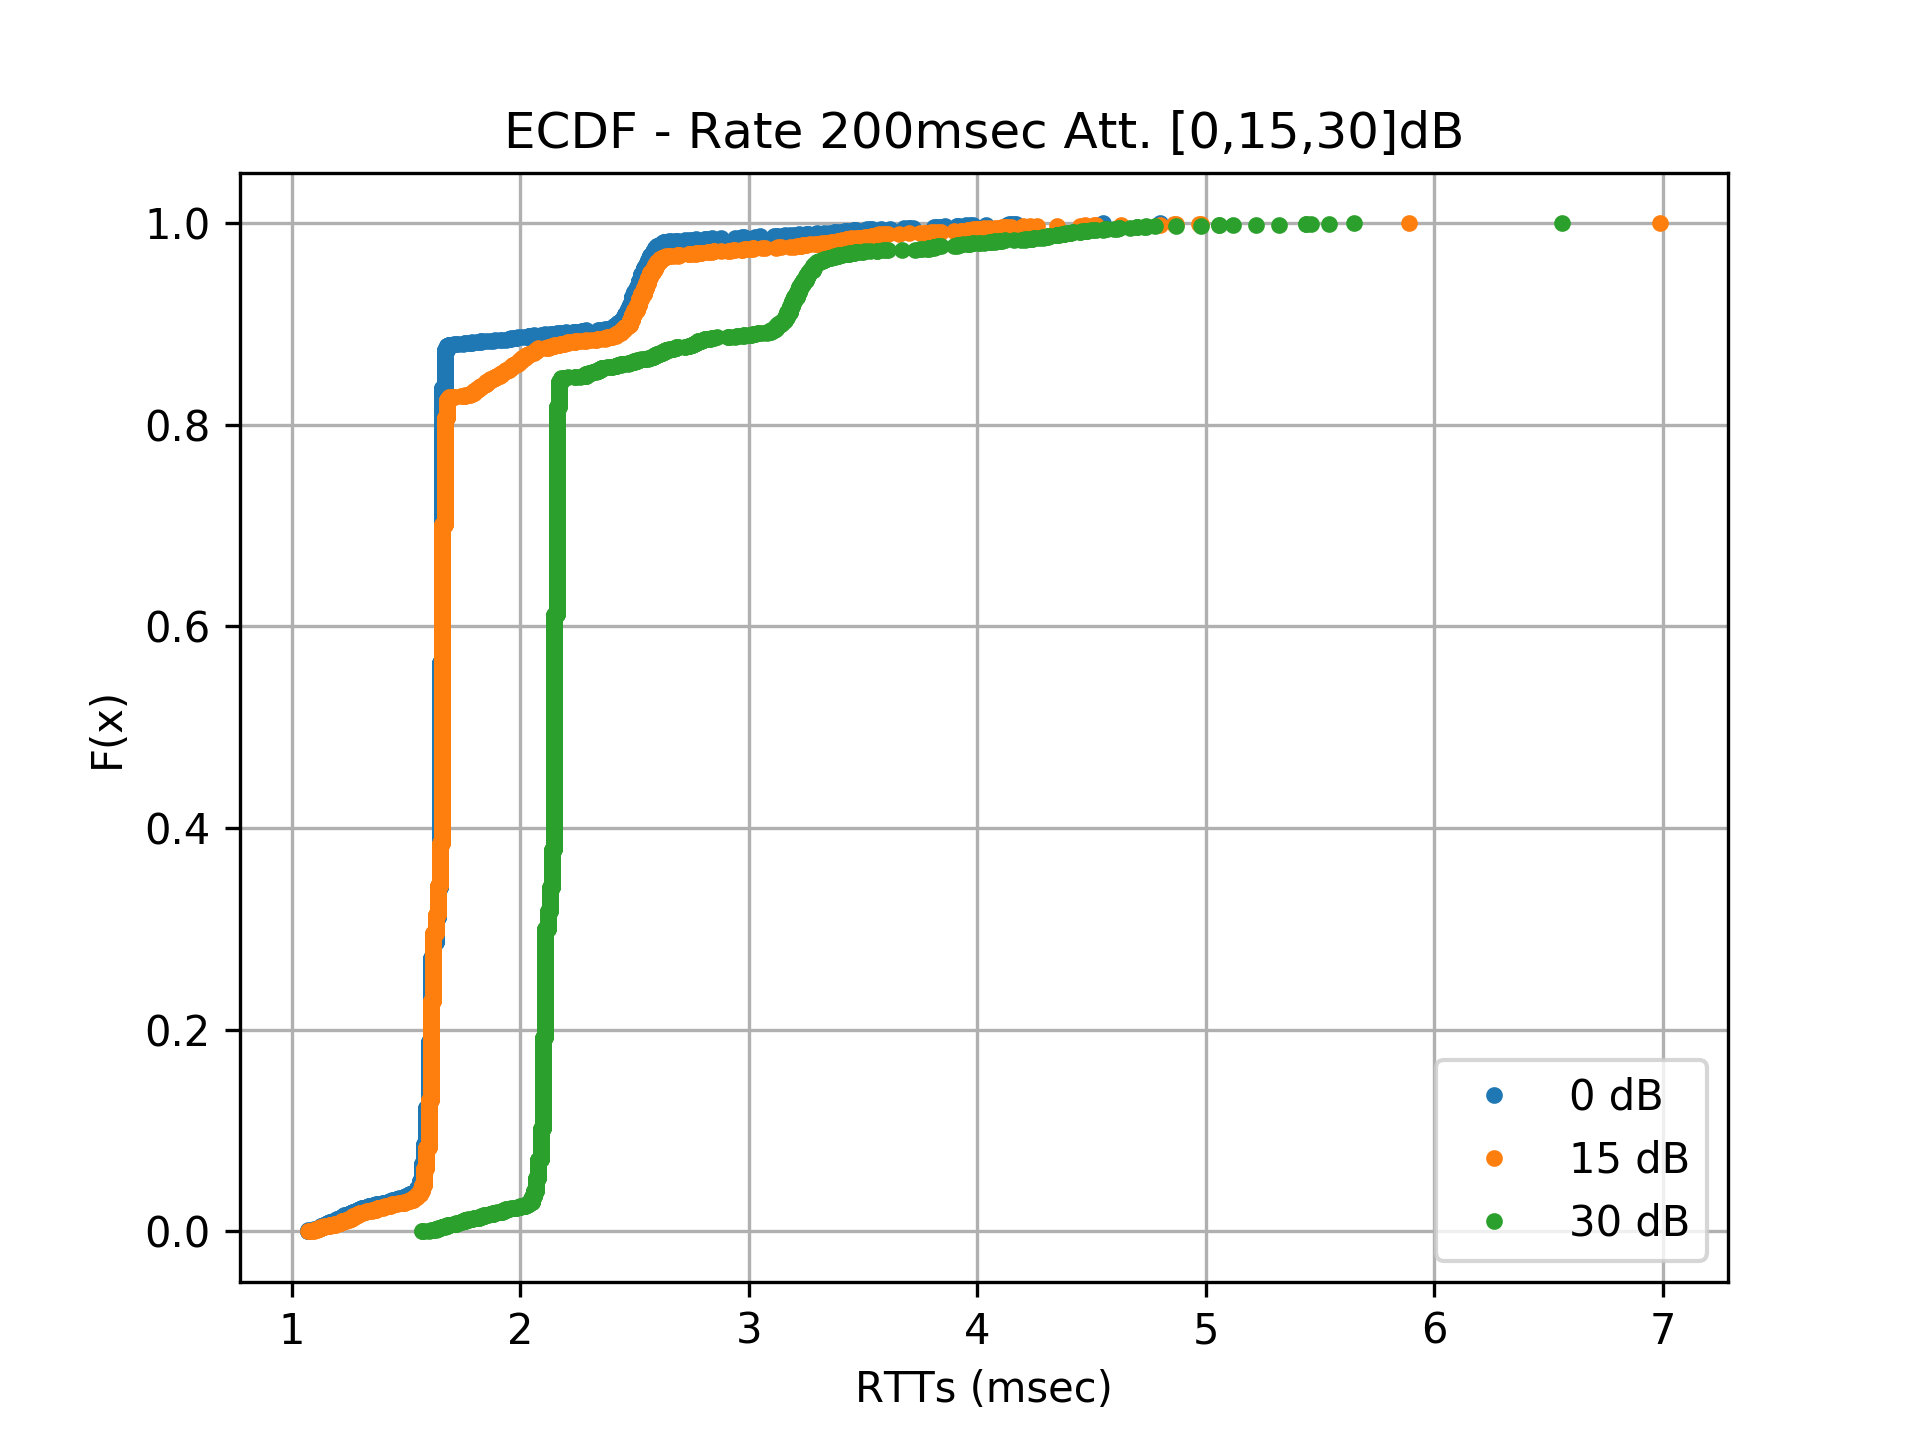
\includegraphics[width=.9\textwidth]{Rates_Atts/Rate200msecAtt_[0,15,30]dB}
		\caption{Rate 200 msec - Att. [0,15,30] dB}
		\label{fig:rate_200msec_Att_0_15_30dBm}
	\end{subfigure}
	\caption{RTT ECDFs for Attenuation and Probing Rate in Testbed}
\end{figure*}
\newpage